\chapter{Analytical Description Nozzle Shapes}
\label{ch:Analytical}

\noindent Now the method which will be investigated further is decided, an analytical description and in depth study is done regarding the literature of nozzle shapes. All of this chapter is found in \cite{Lee+} where a distinguishment is made between four options: Round jet, round plume, plane jet and plane plume. The case of a plane jet is more extensive featured, where the other are shorter elaborated. This because the method complies with each other in all cases, with a few differences, and all literature is found in \cite{Lee+} as said before. \newline 

\noindent For all four cases, the entrainment coefficient $(\alpha_G)$ and velocity- to concentration width ratio $(\lambda_r)$ are described and determined. The entrainment coefficient relates to the spreading rate $(\beta_G)$ which is determined by experiments. The experiment setup is described in chapter \ref{ch:test_setup}. Section \ref{sec:summary_entrainment} gives a summary of all relations needed for the experiments.

\nomenclature[Z]{ZFE}{Zone of Flow Establishment}
\nomenclature[Z]{ZEF}{Zone Established Flow}

\newpage
\section{Jets}
\label{sec:planejet}



%%%%%%%%%%%%%%%%%%%%%%%%%%%%%%%%%%%%%%%%%%%%%%%%%%%%%%%%%%%%%%%%%%%%%%%%%%%%%%%%%%%%%%%%%%%%%%%%%%%%%%%%%%%%%%%%%%%%%%%%%%%%%%%%%%%%%%%%%%%%%%%%%%%%%%%%%%%%%%%%%%%%%%%%%%%%%%%%%%%%%%%%%%%%%%%%%%%%%%%%%%%%%%%%%%%%%%%%%%%%%%%%%%%%%%%%%%%%%%%%%%%%%%%%%%%%%%%%%%%%%%%%%%%%%%%%%%%%%%%%%%%%%%%%%%%%%%%%%%%%%%%%%%%%%%%%%%%%%%%%%%%%%%%%%%%%%%%%%%%%%%%%%%%%%%%%%%%%%%%%%%%%%%%%%%%%%%%%%%%%%%%%%%%%%%%%%%%%%%%%%%%%%%%%%%%%%%%%%%%%%%%%%%%%%%%%%%%%%%%%%%%%%%%%%%%%%%%%%%%%%%%%%%%%%%%%%%%%%%%%%%%%%%%%%%%%%%%%%%%%%%%%%%%%%%%%%%%%%%%%%%

\subsection{Plane Jet}

% zone of establishment
Looking at the inflow of a continuous source of momentum two different zones are noted: Zone of Flow Establishment (ZFE) and Zone Established Flow (ZEF) which can be seen in figure \ref{fig:zone_plane} in case of a plane outflow shape. 



\begin{figure}[ht!]
    \centering
    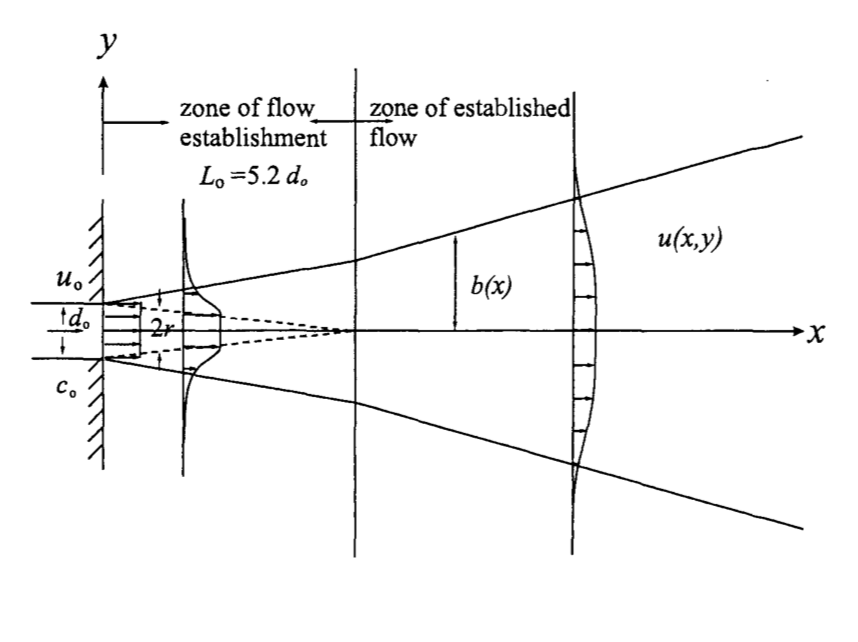
\includegraphics[width=0.6\textwidth]{Images/Plane_jet_flow.png}
    \caption{Zone of Flow Establishment (ZFE) and Zone Established Flow (ZEF) in case of a plane jet}
    \label{fig:zone_plane}
\end{figure}

\noindent The velocity and concentration in the potential core of the ZFE are constant. Surrounding the potential core is the mixing layer. The exchange of momentum between the core and the surrounding fluid across the mixing layer leads to the profiles in the mixing layer as follows:

\begin{equation}
\begin{split}
    & u(x,y) = u_0 * exp [\frac{- (y-r)^2}{b^2}];y > r  \\     
    & c(x,y) = c_0 * exp [\frac{- (y-r)^2} { (\lambda_r b)^2}] ; y > r
    \end{split}
\end{equation}
\begin{equation}
\begin{split}
    & u(x,y) = u_0; y < r \\     
    & c(x,y) = c_0; y < r
    \end{split}
    \label{eq:gaus}
\end{equation}

\noindent where r(x) = half-width of the potential core, b(x) = width of the mixing layer, u(x,y) = velocity, c(x,y) = concentration, and y = lateral distance from the center line. The parameter $\lambda_r$ is introduced to account for the difference between the diffusion of mass and diffusion of momentum. The width of the concentration profile $\lambda_r$b(x) is generally wider than the width of the velocity profiles b(x) at the end of the potential core (r $\rightarrow$ 0). \newline

\noindent In the Zone of Established Flow (ZEF),when the turbulence has penetrated to the centerline, the velocity and concentration distributions are self-similar (this means the profiles at different x all look similar in shape, so that if the profiles at different x are scaled properly, all these should collapse onto one curve), and can be well approximated by Gaussian distributions:

\begin{equation}
\begin{split}
    &u(x,y) = u_m * exp [\frac{-y^2}{b^2}] ; x > 5.2d_0 \\   
    &c(x,y) = c_m * exp [\frac{-y^2} {(\lambda_r b)^2}] ; x > 5.2d_0
    \end{split}
    \label{eq:gaus_2}
\end{equation}

\noindent where $u_m$(x) and $c_m$(x) are the velocity and concentration maxima along the centerline. The width of the jet, b(x), is defined at a lateral location where the x-component of the velocity is equal to 1/e of the centerline value. Experimental measurements of plane jet by \cite{Albertson}, \cite{Miller} and \cite{Bradbury} found the jet spreads linearly with a growth rate $\frac{db}{dx} \simeq 0.1$.\newline

%%%%%%%%%%%%%%%%%%%%%%%%%%%%%%%%%%%%%%%%%%%%%%%%%%%%%%%%%%%%%%%%%%%%%%%%%%%%%%%%%%%%%%%%%%%%%%%%%%%%%%%%%%%%%%%%%%%%%%%%%%%%%%%%%%%%%%%%%%%%%%%%%%%%%%%%%%%%%%%%%%%%%%%%%%%%%%%%%%%%%%%%%%%%%%%%%%%%%%%%%%%%%%%%%%%%%%%%%%%%%%%%%%%%%%%%%%%%%%%%%%%%%%%%%%%%%%%%%%%%%%%%%%%%%%%%%%%%%%%%%%%%%%%%%%%%%%%%%%%%%%%%%%%%%%%%%%%%%%%%%%%%%%%%%%%%%%%%%%%%%%%%%%%%%%%%%%%%%%%%%%%%%%%%%%%%%%%%%%%%%%%%%%%%%%%%%%%%%%%%%%%%%%%%%%%%%%%%%%%%%%%%%%%%%%%%%%%%%%%%%%%%%%%%%%%%%%%%%%%%%%%%%%%%%%%%%%%%%%%%%%%%%%%%%%%%%%%%%%%%%%%%%%%%%%%%%%%%%%%%%%

\subsubsection{Governing Equations}

The governing equations for the steady incompressible turbulent mean flow of the jet are the continuity equation (\ref{eq:cont}), the momentum equations (\ref{eq:mom}) and the mass conservation equation (\ref{eq:mass}). The reference frame is the same as figure \ref{fig:zone_plane}.

\begin{equation}
    \frac{\partial u}{\partial x} + \frac{\partial v}{\partial y} = 0
    \label{eq:cont}
\end{equation}

\begin{equation}
\begin{split}
    & \rho u\frac{\partial u}{\partial x} + \rho v \frac{\partial u}{\partial y} = - \frac{\partial p}{\partial x} - \frac{\partial \rho \overline{u'^2}}{\partial x} - \frac{\partial \rho \overline{u'v'}}{\partial y} \\
    & \rho u\frac{\partial v}{\partial x} + \rho v \frac{\partial v}{\partial y} = - \frac{\partial p}{\partial v} - \frac{\partial \rho \overline{u'v'}}{\partial x} - \frac{\partial \rho \overline{v'^2}}{\partial y}
    \end{split}
    \label{eq:mom}
\end{equation}

\begin{equation}
  u \frac{\partial c}{\partial x} + v \frac{\partial c}{\partial y} = - \frac{\partial \overline{u'c'}}{\partial x} - \frac{\partial \overline{v'c'}}{\partial y}
    \label{eq:mass}
\end{equation} 

\noindent where (u, v) = mean velocity, c = mean concentration (mass per unit volume), p = pressure, and $\rho$ = fluid density; the prime denote the turbulent fluctuations and overbar the time average of the fluctuations. The boundary conditions for a free jet are shown in equation \ref{eq:freejet} for $y \rightarrow \pm \infty$. With these boundary conditions the jet is assumed to be free from solid boundary and ambient current effects.
\begin{equation}
\begin {split}
   &u \rightarrow 0  \\
 &\overline{u'v'} \rightarrow 0 \\
 &\overline{u'c'} \rightarrow 0 
    \end{split}
    \label{eq:freejet}
\end{equation}

\noindent Furthermore, since b $\ll$ x, by continuity v $\ll$ u and $\frac{\partial}{\partial x} \ll \frac{\partial }{\partial y}$ , the
pressure $p$ is approximately constant and $\frac{\partial p}{\partial x} \approx \frac{\partial p}{\partial y} \approx 0$. Hence, 

\begin{equation}
    p + \rho \overline{v'^2} \simeq p_\infty
\end{equation}
from the boundary-layer approximation of the y-momentum equation (\ref{eq:mom}). Which leaves three equations which are subjected to the same boundary conditions as specified before. Thus there are three variables of the mean flow (u,v,c) and three governing equations (\ref{eq:cont}, \ref{eq:mom} in x direction and \ref{eq:mass}). But the turbulent covariances ($\overline{u'v'}, \overline{v'c'}$) are the additional unknowns due to the separation of the flow into mean and fluctuation parts. Therefore a turbulence model must be introduced to relate these covariances with the mean flow. \newline


%%%%%%%%%%%%%%%%%%%%%%%%%%%%%%%%%%%%%%%%%%%%%%%%%%%%%%%%%%%%%%%%%%%%%%%%%%%%%%%%%%%%%%%%%%%%%%%%%%%%%%%%%%%%%%%%%%%%%%%%%%%%%%%%%%%%%%%%%%%%%%%%%%%%%%%%%%%%%%%%%%%%%%%%%%%%%%%%%%%%%%%%%%%%%%%%%%%%%%%%%%%%%%%%%%%%%%%%%%%%%%%%%%%%%%%%%%%%%%%%%%%%%%%%%%%%%%%%%%%%%%%%%%%%%%%%%%%%%%%%%%%%%%%%%%%%%%%%%%%%%%%%%%%%%%%%%%%%%%%%%%%%%%%%%%%%%%%%%%%%%%%%%%%%%%%%%%%%%%%%%%%%%%%%%%%%%%%%%%%%%%%%%%%%%%%%%%%%%%%%%%%%%%%%%%%%%%%%%%%%%%%%%%%%%%%%%%%%%%%%%%%%%%%%%%%%%%%%%%%%%%%%%%%%%%%%%%%%%%%%%%%%%%%%%%%%%%%%%%%%%%%%%%%%%%%%%%%%%%%%%%



\subsubsection{Integral Turbulence equations} 
A one-dimensional procedure to achieve the turbulent closure of the problem is to integrate across the turbulent jet. First, the x-momentum equation is re-written to a conservative form. Since, 

\begin{equation}
    \rho u \frac{\partial u}{\partial x} + \rho v \frac{\partial u}{\partial y} = \frac{\partial \rho u^2}{\partial x} + \frac{\partial \rho uv}{\partial y} - \rho u (\frac{\partial u}{\partial x} + \frac{\partial v}{\partial y})
\end{equation}
\noindent The x-momentum equation (\ref{eq:mom}) becomes:

\begin{equation}
    \frac{\partial \rho u^2}{\partial x} + \frac{\partial \rho uv}{\partial y} + \frac{\partial \rho \overline{u^2}}{\partial x} - \frac{\partial \rho \overline{v^2}}{\partial x} = - \frac{\partial \rho \overline{u'v'}}{\partial y}
    \label{eq:xmom_cons}
\end{equation}

\noindent Using the boundary condition and integrating across the jet, from y = - $\infty$ to y = + $\infty$, equation \ref{eq:xmom_cons} becomes:

\begin{equation}
\begin{split}
    &\frac{d}{dx} \int_{-\infty}^{\infty} \frac{\partial \rho u^2}{\partial x} + \frac{\partial \rho uv}{\partial y} + \frac{\partial \rho \overline{u^2}}{\partial x} - \frac{\partial \rho \overline{v^2}}{\partial x} = \int_{-\infty}^{\infty} (- \frac{\partial \rho \overline{u'v'}}{\partial y})dy \\
    &\frac{d}{dx} \int_{-\infty}^{\infty} \rho u^2 + \rho (\overline{u'^2} - \overline{v'^2})dy + [\rho uv]_{-\infty}^{\infty} = [- \rho \overline{u'v'}]_{-\infty}^{\infty} \\
    &\frac{d}{dx} \int_{-\infty}^{\infty} [\rho u^2 + \rho (\overline{u'^2} - \overline{v'^2})]dy = 0 
    \end{split}
    \label{eq:int}
\end{equation}
\noindent Equation \ref{eq:int} shows that the momentum flux is preserved and the plane jet is a line source of momentum flux. If $M$ is the momentum flux per unit length, equation \ref{eq:int} becomes:

\begin{equation}
    M= \int_{-\infty}^{\infty} [\rho u^2 + \rho (\overline{u'^2} - \overline{v'^2})dy] 
\end{equation}

\noindent Similarly for the mass conservation, using previous steps shown for the momentum equation, finally we get:

\begin{equation}
   \frac{d}{dx}\int_{-\infty}^{\infty} [uc + \overline{u'c'}]dy = [- \overline{v'c'}]_{-\infty}^{\infty}
   \label{eq:mass_flux}
\end{equation}
\noindent The right hand side would be zero if the concentration c is the concentration excess above its value in the ambient and hence that the excess mass flux is constant. If $\Gamma$ is this excess mass flux per unit length of the plane jet, equation \ref{eq:mass_flux} becomes:

\begin{equation}
   \Gamma = \int_{-\infty}^{\infty} [uc + \overline{u'c'}]dy
\end{equation}

\noindent Measurements show that the two turbulence quantities in equation \ref{eq:int} are of the same order \citep{Miller}. If the longitudinal fluxes due to turbulent advection are ignored we get:

\begin{equation}
    M \approx \int_{-\infty}^{\infty} [\rho u^2] dy
\end{equation}
\begin{equation}
    \Gamma \approx \int_{-\infty}^{\infty}  [uc]dy
\end{equation}
\noindent These approximated form of equations, since the parts of fluxes due to turbulent advection are ignored, are used in the next sections. \newline \newline













\subsubsection{Eulerian turbulence model} 
The turbulence model of the turbulent jet is based on the assumption of the Gaussian profiles, shown in equations \ref{eq:gaus} \& \ref{eq:gaus_2}. In this subsection, the calculations for the ZEF are considered. Based on the velocity- and concentration profiles in equation \ref{eq:gaus_2}, the specific or kinematic momentum flux ($M/\rho$) and the mass flux are functions of the width of the jet ($b$), the maximum velocity ($u_m$) and the maximum concentration ($c_m$) as follows:

\begin{equation}
    \frac{M}{\rho} = \int_{-\infty}^{\infty} [u^2] dy = \sqrt{\frac{\pi}{2}} u_m^2 b
\end{equation}

\begin{equation}
    \Gamma = \int_{-\infty}^{\infty} [uc] dy = \sqrt{\frac{\pi\lambda_r^2}{1+\lambda_r^2}}u_m c_m b
\end{equation}

\noindent Equating the expressions in the above equations to the flux at the source, $M = u_0^2 d_0$ and $\Gamma = u_0 c_0 d_0$ and assuming $b=\beta_G x$, a relation between the centerline velocity ($\frac{u_m}{u_o}$) and centerline concentration ($\frac{c_m}{c_0}$) can be distinguished. 

\begin{equation}
    \frac{u_m}{u_o} = \sqrt{\frac{2 d_0}{\pi \beta_G x}}
\end{equation}
\begin{equation}
    \frac{c_m}{c_o} = \sqrt{\frac{1+\lambda_r^2 d_o}{\lambda_r^2 \beta_G \sqrt{2\pi} x}}
\end{equation}


\nomenclature[G]{$\lambda_r$}{Ratio of concentration to velocity width \nomunit{[-]}}
\nomenclature[G]{$\beta_G$}{Spreading rate based on Gaussian profile \nomunit{[-]}}
\nomenclature[A]{$d_0$}{Plane/slot width \nomunit{[$m$]}}
\nomenclature[A]{$S$}{Centerline dilution ratio \nomunit{[-]}}
\nomenclature[G]{$\alpha_G$}{Entrainment coefficient based on Gaussian velocity profile\nomunit{[-]}}

\noindent where $\lambda_r$ is the ratio of concentration to velocity width, $b$ is the half-width of jet/plume, $\beta_G$ the spreading rate based on the Gaussian velocity profile and $d_0$ the plane width. The subscripts ($_m , _0$) denote the centerline maximum and source. The volume flux (per unit length of the plane exit) $Q$ at a distance $x$ from the source is greater than the volume flux $Q_0$, which is the jet dilution in order to fulfill the momentum conservation.

\begin{equation}
    Q = \int_{-\infty}^{\infty} [u] dy = \sqrt{\pi} u_m b = [{\sqrt{2\pi} \beta_G }]^\frac{1}{2} [\frac{x}{d_0}]^\frac{1}{2} u_0 d_0
    \label{eq:Q}
\end{equation}

\noindent With the centerline dilution ratio:

\begin{equation}
    S = \frac{Q}{Q_0} = [\sqrt{2\pi} \beta_G]^\frac{1}{2} [\frac{x}{d_0}]^\frac{1}{2}
\end{equation}

\noindent The jet spread rate $\beta_G$ has to be determined experimentally. The ratio between velocity and concentration width $\lambda_r$ is determined in experiments by \cite{Kotsovinos} which give a value of $\lambda_r = 1.35$. \newline 

\noindent \textbf{Entrainment Hypothesis} \newline
The closure problem can also be looked at a different way. Integrating the continuity equation across the jet:

\nomenclature[A]{$v_e$}{Entrainment velocity \nomunit{[$m/s$]}}

\begin{equation}
    \frac{dQ}{dx} = \frac{d}{dx} \int_{-\infty}^{\infty} [u] dy = [-v]_\infty^\infty = 2v_e
    \label{eq:Qx}
\end{equation}

\noindent Where $v_e (= |v|_{y=\pm\infty})$ is the entrainment velocity. In this case, the closure problem says something about the entrainment velocity and its relationship to the local jet characteristics. By integrating equation \ref{eq:Q} and using the solution for $Q(x)$:

\begin{equation}
\begin{split}
     \frac{dQ}{dx} & =  \frac{(\sqrt{2\pi}\beta_G)^\frac{1}{2}}{2} u_0 (\frac{d_0}{x}) \\
    & = 2(\frac{\sqrt{\pi \beta_G}}{4}) u_m
    \end{split}
    \label{eq:Qx_2}
\end{equation}

\noindent Comparing equation \ref{eq:Qx} \& \ref{eq:Qx_2} it shows that the entrainment velocity is proportional to the local jet centerline velocity. This means that the closure problem could be solved by beginning the assumption that $v_e = \alpha_G u_m$, where $\alpha$ is the entrainment coefficient, and solve the continuity, momentum ans mass conservation equations. In many buoyant jet problems, turbulent closure can be solved by this entrainment hypothesis proposed by \cite{Morton}. The entrainment factor can be obtained by experiments and depends on the spreading rate $\beta_G$ in the case of 2D plane jet.

\begin{equation}
    \alpha_G = \frac{\sqrt{\pi}}{4} \beta_G
\end{equation}



%%%%%%%%%%%%%%%%%%%%%%%%%%%%%%%%%%%%%%%%%%%%%%%%%%%%%%%%%%%%%%%%%%%%%%%%%%%%%%%%%%%%%%%%%%%%%%%%%%%%%%%%%%%%%%%%%%%%%%%%%%%%%%%%%%%%%%%%%%%%%%%%%%%%%%%%%%%%%%%%%%%%%%%%%%%%%%%%%%%%%%%%%%%%%%%%%%%%%%%%%%%%%%%%%%%%%%%%%%%%%%%%%%%%%%%%%%%%%%%%%%%%%%%%%%%%%%%%%%%%%%%%%%%%%%%%%%%%%%%%%%%%%%%%%%%%%%%%%%%%%%%%%%%%%%%%%%%%%%%%%%%%%%%%%%%%%%%%%%%%%%%%%%%%%%%%%%%%%%%%%%%%%%%%%%%%%%%%%%%%%%%%%%%%%%%%%%%%%%%%%%%%%%%%%%%%%%%%%%%%%%%%%%%%%%%%%%%%%%%%%%%%%%%%%%%%%%%%%%%%%%%%%%%%%%%%%%%%%%%%%%%%%%%%%%%%%%%%%%%%%%%%%%%%%


\newpage
\subsection{Round Jet}
% zone of establishment 
In case of a round shape and a continuous source of momentum, the ZFE and ZEF are slightly different, which can be seen in figure \ref{fig:zone_round}.

\begin{figure}[H]
    \centering
    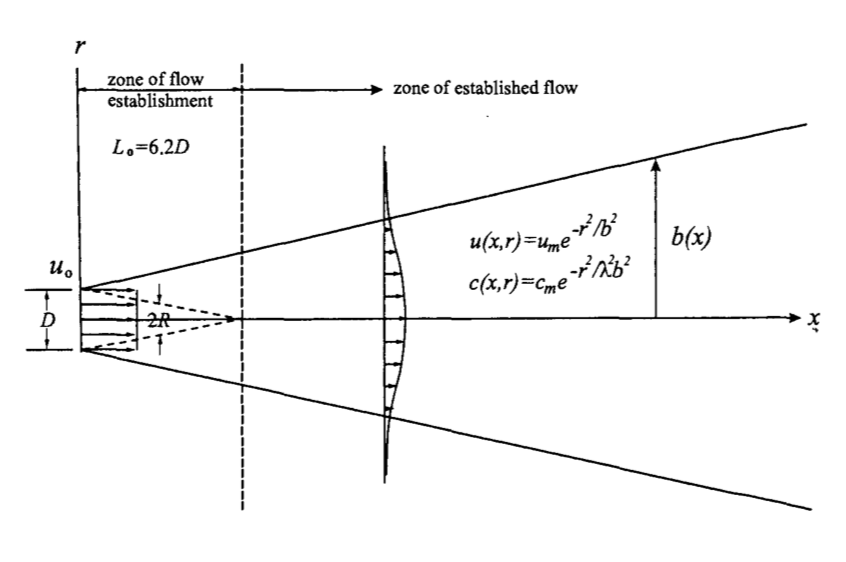
\includegraphics[width=0.6\textwidth]{Images/Round_Jet_flow.png}
    \caption{Zone of Flow Establishment (ZFE) and Zone Established Flow (ZEF) in case of a round jet}
    \label{fig:zone_round}
\end{figure}

\noindent The general experimental features described in section \ref{sec:planejet} also apply for the case of a round jet. The diffusion thickness spreads linearly, static pressure is approximated constant and so the same boundary layer approximations can me made. Again the velocity and concentration profiles can be described according to \ref{fig:zone_round}. \newline

\noindent In the ZFE, $x \leq 6.2D$:
\begin{equation}
    \begin{split}
        & u = u_0 ; r \leq R \\
        & c = c_0 ; r \leq R
    \end{split}
\end{equation}

\begin{equation}
    \begin{split}
        & u = u_0 * exp [ - \frac{(r-R)^2}{b^2}] ; r \geq R \\
        & c = c_0 * exp [ - \frac{(r-R)^2}{\lambda_r^2 b^2}] ; r \geq R
    \end{split}
\end{equation}

\noindent For $x \geq 6.2D$ also known as the ZEF:

\begin{equation}
    \begin{split}
        & u = u_m * exp [ - (\frac{r}{b})^2] \\
        & c = c_m * exp [ - (\frac{r}{\lambda_r b})^2]
    \end{split}
\end{equation}

\noindent Where (x,r) are the streamwise and radial coordinates and $u_m(x)$ and $c_m(x)$ are the centerline maximum velocity and concentration. Also the assumption holds that the turbulent round jet spreads linearly with $b = \beta_G x$. Because the round jet is a 3D case, the momentum-, continuity- and mass conservation equations are changed to a (x,r) coordinate system. Showing below are the continuity equation (\ref{eq:cont_polar}), momentum equation in x-direction (\ref{eq:mom_polar}) and the mass conservation equation (\ref{eq:mass_polar}).

\begin{equation}
    \rho \frac{\delta u}{\delta x} + \rho \frac{1}{r}\frac{\delta}{\delta r} (rv) = 0\
    \label{eq:cont_polar}
\end{equation}

\begin{equation}
    \rho u \frac{\delta u}{\delta x} + \rho v \frac{\delta u}{\delta r} = - \frac{1}{r}\frac{\delta}{\delta r}(r\rho \overline{u'v'})
    \label{eq:mom_polar}
\end{equation}


\begin{equation}
    u \frac{\delta c}{\delta x} + v \frac{\delta d}{\delta r} = - \frac{1}{r}\frac{\delta}{\delta r} (r\overline{v'c'})
    \label{eq:mass_polar}
\end{equation} \newline

\noindent \cite{Lee+} evaluated the derivation the same way as with a plane jet, by solving the momentum flux the same way showed in section \ref{sec:planejet} and so find the centerline velocity ($\frac{u_m}{u_0}$), concentration ($\frac{c_m}{c_0}$) and dilution ($S$). $\lambda_r$ is determined in experiments by \cite{Papanicolaou+} and showed a value of $\lambda_r = 1.2$ in case of a round jet.

\subsubsection{Entrainment Hypothesis} 
Same as the plane jet, the entrainment hypothesis is applicable for a round jet. By using the same method described for the plane jet, and so integrate the continuity equation across the jet, it can be shown that:

\begin{equation}
    \frac{dQ}{dx} = \frac{d}{dx} (\pi u_m b^2) = 2\pi(rv) = Q_e
\end{equation} \newline

\noindent Where the right hand side represents the local entrainment flux into the jet. By defining the inflowing entrainment velocity at r = b as the entrainment velocity ($v_e$) and use the entrainment hypothesis as shown in section \ref{sec:planejet}, the entrainment velocity is assumed to be proportional to the centerline velocity by the entrainment coefficient $\alpha$. Similar to the 2D plane case, it can be shown that the entrainment coefficient depends on the spreading rate, in the case of a 3D round jet.

\begin{equation}
    \alpha_G = \frac{\beta_G}{2}
\end{equation}





%%%%%%%%%%%%%%%%%%%%%%%%%%%%%%%%%%%%%%%%%%%%%%%%%%%%%%%%%%%%%%%%%%%%%%%%%%%%%%%%%%%%%%%%%%%%%%%%%%%%%%%%%%%%%%%%%%%%%%%%%%%%%%%%%%%%%%%%%%%%%%%%%%%%%%%%%%%%%%%%%%%%%%%%%%%%%%%%%%%%%%%%%%%%%%%%%%%%%%%%%%%%%%%%%%%%%%%%%%%%%%%%%%%%%%%%%%%%%%%%%%%%%%%%%%%%%%%%%%%%%%%%%%%%%%%%%%%%%%%%%%%%%%%%%%%%%%%%%%%%%%%%%%%%%%%%%%%%%%%%%%%%%%%%%%%%%%%%%%%%%%%%%%%%%%%%%%%%%%%%%%%%%%%%%%%%%%%%%%%%%%%%%%%%%%%%%%%%%%%%%%%%%%%%%%%%%%%%%%%%%%%%%%%%%%%%%%%%%%%%%%%%%%%%%%%%%%%%%%%%%%%%%%%%%%%%%%%%%%%%%%%%%%%%%%%%%%%%%%%%%%%%%%%%%


\section{Plumes}

\subsection{Plane plume}
\noindent The flow generated by a line source of buoyancy is called a plane plume. The flow in this plume is governed by the buoyancy flux per unit length of the source.  Consider the flow generated by a line source of buoyancy at z=0, in stagnant ambient fluid of constant density $\rho_a$. The motion is sustained by a steady constant buoyancy flux $F_0 = \int_\infty^\infty \frac{\Delta \rho}{\rho} gw dy$ at z=0. Here the continuity-, momentum- and mass conservation equations for the plume are described in the y-z plane, where z is upward positive from the source.

\begin{equation}
    \frac{\delta w}{\delta z} + \frac{\delta v}{\delta y} = 0
\end{equation}

\begin{equation}
    w\frac{\delta w}{\delta z} + v \frac{\delta w}{\delta y} = -\frac{\delta \overline{w'v'}}{\delta y} - \frac{\rho - \rho_a}{\rho_a}g
\end{equation}

\begin{equation}
    w\frac{\delta c}{\delta z} + v\frac{\delta c}{\delta y} = - \frac{\delta \overline{v'c'}}{\delta y}
\end{equation}\newline

\noindent By again assuming a linear spreading rate with $\beta = \frac{dB}{dz}$, experiments from \cite{Kotsovinos} showed a relation between the entrainment coefficient and the spreading rate as follow, based on the Gaussian velocity profile for a plane plume. Next to that, a value of $\lambda_r = 1.35$ in case of a plane plume.

\begin{equation}
    \alpha_G = \frac{\sqrt{\pi}}{2} \beta_G
\end{equation}

%%%%%%%%%%%%%%%%%%%%%%%%%%%%%%%%%%%%%%%%%%%%%%%%%%%%%%%%%%%%%%%%%%%%%%%%%%%%%%%%%%%%%%%%%%%%%%%%%%%%%%%%%%%%%%%%%%%%%%%%%%%%%%%%%%%%%%%%%%%%%%%%%%%%%%%%%%%%%%%%%%%%%%%%%%%%%%%%%%%%%%%%%%%%%%%%%%%%%%%%%%%%%%%%%%%%%%%%%%%%%%%%%%%%%%%%%%%%%%%%%%%%%%%%%%%%%%%%%%%%%%%%%%%%%%%%%%%%%%%%%%%%%%%%%%%%%%%%%%%%%%%%%%%%%%%%%%%%%%%%%%%%%%%%%%%%%%%%%%%%%%%%%%%%%%%%%%%%%%%%%%%%%%%%%%%%%%%%%%%%%%%%%%%%%%%%%%%%%%%%%%%%%%%%%%%%%%%%%%%%%%%%%%%%%%%%%%%%%%%%%%%%%%%%%%%%%%%%%%%%%%%%%%%%%%%%%%%%%%%%%%%%%%%%%%%%%%%%%%%%%%%%%%%%%

\subsection{Round plume}
The round plume is produced by a steady and continuous source of buoyancy. In the case of the jet, the velocity- $w(z,r)$ and concentration $c(z,r)$ field of the plume are calculated as function of upward direction $z$ and radial direction $r$. The round plume good distributed by Gaussian profiles, which simplifies the problem to the prediction of the maximum velocity $(w_m)$ the width $(b)$ and the maximum concentration $(c_m)$ as a function of the upward distance z from the source.


\begin{figure}[ht!]
    \centering
    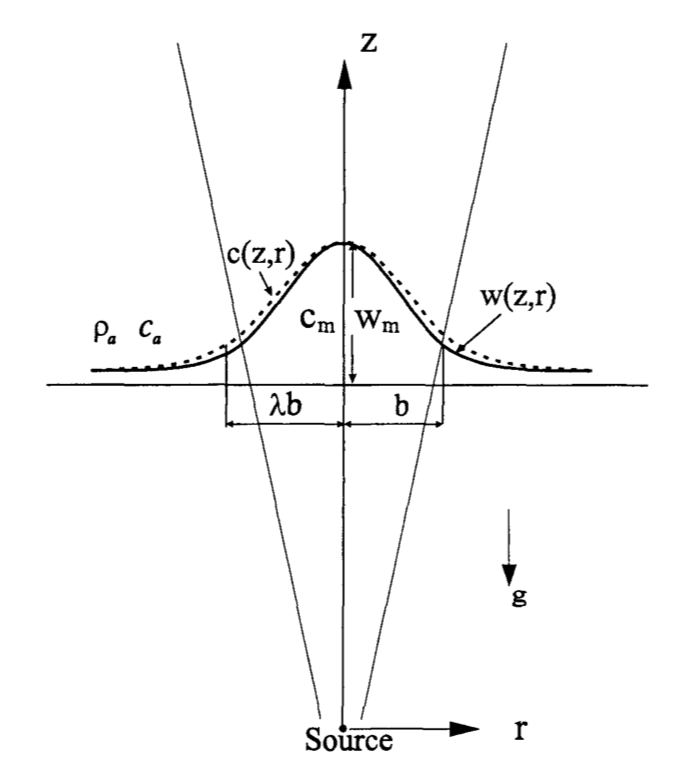
\includegraphics[width=0.4\textwidth]{Images/Round_plume.png}
    \caption{Mean velocity- and concentration profiles in case of round plume. The width of the concentration profile is noted by $\lambda b$ where $b$ is the width of the velocity profile}
    \label{fig:round_plume}
\end{figure}

\nomenclature[G]{$\rho_{amb}$}{Mass density of ambient fluid \nomunit{[$kg/m^3$]}}

\newpage
\noindent Neglecting effects of initial momentum flux and the size of the source, the width of the plume ($b$) depends on its buoyancy flux at the source $B_0$, the ambient fluid density $\rho_{amb}$ and the distance from the source $z$. Same as seen before, the relation holds that the plume spreads linearly with $b = \beta_G z$. The profile shown in figure \ref{fig:round_plume} relates to the following velocity- and concentration profiles (eq \ref{eq:wc}) in the established flow, where the velocity the width of the plume $(b)$ is defined by location with velocity $e^{-1}*w_m$.

\begin{equation}
    \begin{split}
        & w(z,r) = w_m(z) e^{-(\frac{r}{b})^2} \\
        & c(z,r) = c_m(z) e^{-(\frac{r}{\lambda b})^2}
    \end{split}
    \label{eq:wc}
\end{equation}

\noindent The governing continuity- (\ref{eq:cont_plume}), momentum-(\ref{eq:mom_plume}) and mass conservation (\ref{eq:mass_plume}) turbulent incompressible equations in coordinate system (z,r) are defined as follow:

\begin{equation}
    \frac{\delta w}{\delta z} + \frac{1}{r}\frac{\delta}{\delta r} (rv) = 0
    \label{eq:cont_plume}
\end{equation}

\begin{equation}
    \rho(w\frac{\delta w}{\delta z} + v \frac{\delta w}{\delta r}) = - \rho g - \frac{\delta p}{\delta z} - \rho \frac{1}{r}\frac{\delta}{\delta r}(r \overline{w'v'})
    \label{eq:mom_plume}
\end{equation}

\begin{equation}
    w\frac{\delta c}{\delta z} + v \frac{\delta c}{\delta r} = = - \frac{1}{r}\frac{\delta}{\delta r} (r\overline{v'c'})
    \label{eq:mass_plume}
\end{equation}\newline

\noindent Where $w, v$ are the turbulent mean velocities in vertical and radial direction (z,r) and $w', v', c'$ are the velocity and concentration fluctuations. Assuming a hydrostatic pressure distribution $( \frac{\delta p}{\delta z} = - \rho_{amb}*g)$ and adding the Boussinesq approximation, which says that for small densities differences $(\frac{\Delta \rho}{\rho} \ll 1)$ density differences can be neglected and so $\rho \approx \rho_{amb}$, except in terms where the the pressure is multiplied with the gravity acceleration $g$. Using this approximation, the momentum equation (\ref{eq:mom_plume}) becomes:

\begin{equation}
    w \frac{\delta w}{\delta z} + v \frac{\delta w}{\delta r} = - \frac{(\rho - \rho_{amb})}{\rho_{amb}}g - \frac{1}{r}\frac{\delta }{\delta r}(r\overline{w'v'})
\end{equation}

\noindent Same as found in section \ref{sec:planejet}, using integral model equations and the entrainment hypothesis, by solving the volume-, buoyancy- and momentum flux, a relations between the width and entrainment coefficient $(\alpha_G)$ is found. Experiments by \cite{Papanicolaou+} showed a concentration to velocity ratio for a round plume of $\lambda_r = 1.06$, however, a value of $\lambda_r = 1.19$ is suggested for the entire jet and plume range.

\begin{equation}
    b = \frac{6 \alpha_G}{5}z
    \label{eq:alpha_roundplume}
\end{equation}

\noindent By combining equation \ref{eq:alpha_roundplume} and the fact that the plume spreads linearly with $b = \beta_Gz$, an expression for the entrainment coefficient is found in case for a round plume.

\begin{equation}
    \alpha_G = \frac{5\beta_G}{6}
\end{equation}



%%%%%%%%%%%%%%%%%%%%%%%%%%%%%%%%%%%%%%%%%%%%%%%%%%%%%%%%%%%%%%%%%%%%%%%%%%%%%%%%%%%%%%%%%%%%%%%%%%%%%%%%%%%%%%%%%%%%%%%%%%%%%%%%%%%%%%%%%%%%%%%%%%%%%%%%%%%%%%%%%%%%%%%%%%%%%%%%%%%%%%%%%%%%%%%%%%%%%%%%%%%%%%%%%%%%%%%%%%%%%%%%%%%%%%%%%%%%%%%%%%%%%%%%%%%%%%%%%%%%%%%%%%%%%%%%%%%%%%%%%%%%%%%%%%%%%%%%%%%%%%%%%%%%%%%%%%%%%%%%%%%%%%%%%%%%%%%%%%%%%%%%%%%%%%%%%%%%%%%%%%%%%%%%%%%%%%%%%%%%%%%%%%%%%%%%%%%%%%%%%%%%%%%%%%%%%%%%%%%%%%%%%%%%%%%%%%%%%%%%%%%%%%%%%%%%%%%%%%%%%%%%%%%%%%%%%%%%%%%%%%%%%%%%%%%%%%%%%%%%%%%%%%%%%

\section{Jet to plume length}
As shown in equation \ref{eq:lm}, and here as reminder equation \ref{eq:lm2}, \cite{Fischer+} derived a length scale ($l_m$) which states that when $z < l_m$ from the source, a buoyant jet acts as a jet and when $z > l_m$ the buoyant jet acts as a plume. $l_m$ depends on the ratio of initial momentum ($M_0$) and initial buoyancy flux ($B_0$), which both depend on the initial volume flow ($Q_0$) and discharge velocity ($u_0$). Here we can distinguish two cases, a plane- and round jet. An overview of these terms determined by \cite{Lee+} are shown in equations \ref{eq:plane_lm} and \ref{eq:Round_lm}.\newline 

\begin{equation}
\label{eq:lm2}
 l_m = \frac{M_0^{3/4}}{B_{0}^{1/2}}
\end{equation}


\noindent In case of a plane jet:

\begin{equation}
\begin{split}
    & Q_0 =  \frac{1}{2}\sqrt{\pi} *D* u_0 \\
    & M_0 = \frac{1}{2}\sqrt{\frac{\pi}{2}}* D *u_0^2 \\
    & B_0 = Q_0 * g'
  \end{split}  
  \label{eq:plane_lm}
\end{equation}

\noindent In case of a round jet:
\begin{equation}
\begin{split}
    & Q_0 =\frac{\pi}{4} * D^2 * u_0 \\
    & M_0 = Q_0* u_0 \\
    & B_0 = Q_0* g'
  \end{split}  
  \label{eq:Round_lm}
\end{equation}

\noindent Where $g'$ is the specific gravity $\frac{\rho_m - \rho_w}{\rho_w}g$. Note that the plane jet is a 2D case and the round jet is a 3D case.

\nomenclature[A]{$g'$}{Specific gravity \nomunit{[$m/s^2$]}}

%%%%%%%%%%%%%%%%%%%%%%%%%%%%%%%%%%%%%%%%%%%%%%%%%%%%%%%%%%%%%%%%%%%%%%%%%%%%%%%%%%%%%%%%%%%%%%%%%%%%%%%%%%%%%%%%%%%%%%%%%%%%%%%%%%%%%%%%%%%%%%%%%%%%%%%%%%%%%%%%%%%%%%%%%%%%%%%%%%%%%%%%%%%%%%%%%%%%%%%%%%%%%%%%%%%%%%%%%%%%%%%%%%%%%%%%%%%%%%%%%%%%%%%%%%%%%%%%%%%%%%%%%%%%%%%%%%%%%%%%%%%%%%%%%%%%%%%%%%%%%%%%%%%%%%%%%%%%%%%%%%%%%%%%%%%%%%%%%%%%%%%%%%%%%%%%%%%%%%%%%%%%%%%%%%%%%%%%%%%%%%%%%%%%%%%%%%%%%%%%%%%%%%%%%%%%%%%%%%%%%%%%%%%%%%%%%%%%%%%%%%%%%%%%%%%%%%%%%%%%%%%%%%%%%%%%%%%%%%%%%%%%%%%%%%%%%%%%%%%%%%%%%%%%%%%%%%%%%%%%%%


\section{Summary}
\label{sec:summary_entrainment}

Most importantly, from literature and studying \cite{Lee+}, the entrainment coefficient $(\alpha_G)$ and the concentration- to velocity width ratio $(\lambda_r)$ are described and determined in this chapter. An overview for all cases are shown in table \ref{tab:alpha_lambda}.

\begin{table}[ht!]
\begin{tabular}{|c|c|c|c|c|}
\hline
\multicolumn{1}{|l|}{\textbf{}} & \textbf{Round Jet} & \textbf{Round Plume} & \textbf{Plane Jet} & \textbf{Plane Plume} \\ \hline
\textbf{\begin{tabular}[c]{@{}c@{}}Entrainment coefficient \\ $(\alpha_G)$\end{tabular}} & $\frac{\beta_G}{2}$  & $\frac{5}{6}\beta_G$ & $\frac{\sqrt{\pi}}{4}\beta_G$  & $\frac{\sqrt{\pi}}{2}\beta_G$  \\ \hline
\textbf{\begin{tabular}[c]{@{}c@{}}Velocity- to concentration width ratio\\ $(\lambda_r)$\end{tabular}} & \multicolumn{2}{c|}{1.19} & \multicolumn{2}{c|}{1.35} \\ \hline
\textbf{\begin{tabular}[c]{@{}c@{}}Velocity width\\ $(b)$\end{tabular}} & \multicolumn{4}{c|}{$\beta_Gz$} \\ \hline
\end{tabular}
\caption{Overview of all entrainment coefficients and concentration- to velocity width ratios in case of round jet, round plume, plane jet and plane plume}
\label{tab:alpha_lambda}
\end{table}




%Lee_chu boek beschrijven
%verschillende entrainment factoren
%Matlab model Lee_Chu